\newcommand{\wizardhint}{
If this is your first installation, then the setup wizard should appear
when you first run Synergy. The wizard may also appear if we've changed
something or added a new feature.
}

\newcommand{\confighint}{
Once you have installed Synergy on all of your machines, skip to the
"Configure" section of this guide.
}

\section{Install}

Once you have downloaded the latest version of Synergy from our 
downloads page, follow the instructions below.

\subsection{Windows}

To install Synergy on Windows, follow these steps:

\begin{enumerate}
  \item Double click the downloaded installer.
  \item Click "I Agree" to agree to the license.
  \item You can choose an install location, but we recommend you use the default.
  \item Click "Install" to begin the installation.
  \item Once finished, click "Close" to finish the installation.
\end{enumerate}

This is the first screen of the Windows installer:

\begin{figure}[H]
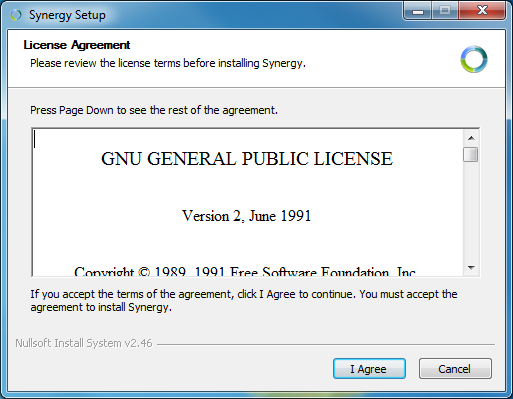
\includegraphics[scale=.75]{graphics/windows-install.png}
\end{figure}

\wizardhint{}
Note that on Windows the wizard may have started behind another window.

\confighint{}

\subsection{Mac OS X}

To install Synergy on Mac OS X, follow these steps:

\begin{enumerate}
  \item Click Finder in your dock.
  \item Select "Applications" from the left.
  \item Open the .dmg file you downloaded.
  \item Drag the Synergy app into Applications.
  \item If prompted, click "Replace".
  \item Find the new Synergy app and double click.
\end{enumerate}

\begin{figure}[H]
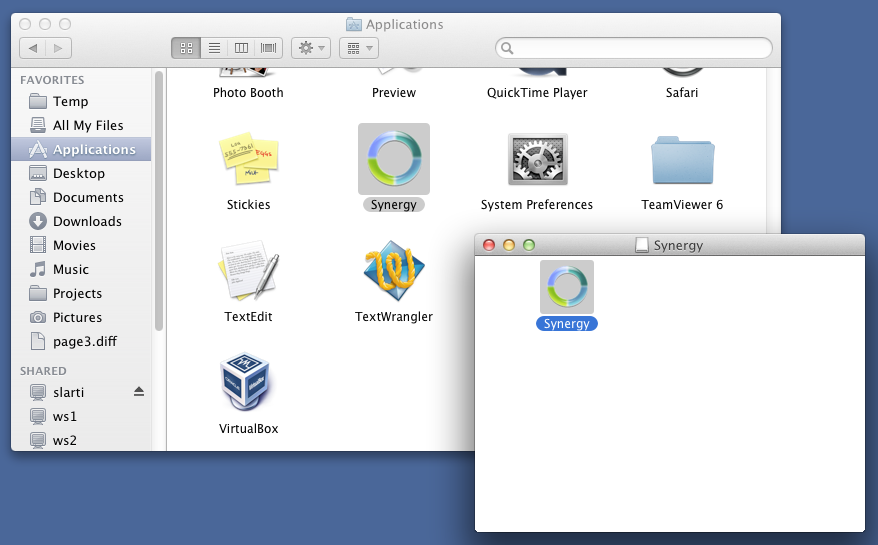
\includegraphics[scale=.65]{graphics/mac-install.png}
\end{figure}

\wizardhint{}

\confighint{}

\subsection{Linux}

To install Synergy on Linux, follow these steps:

\begin{enumerate}
  \item Double click the .deb or .rpm file.
  \item Follow any on-screen install instructions for your distro.
  \item Once complete, you can find the Synergy program in Accessories.
\end{enumerate}

\wizardhint{}

\confighint{}
